% Filename: p2_basic_of_vim@latex_with_vim.tex
% This code is part of LaTeX with Vim.
% 
% Description: LaTeX with Vim is free book about Vim, LaTeX and Git.
% 
% Created: 29.03.12 11:31:01 PM
% Last Change: 29.03.12 11:56:53 PM
% 
% Author: Raniere Gaia Costa da Silva, r.gaia.cs@gmail.com
% Organization:  
% 
% Copyright (c) 2010, 2011, 2012, Raniere Gaia Costa da Silva. All rights 
% reserved.
% 
% This file is license under the terms of a Creative Commons Attribution 
% 3.0 Unported License, or (at your option) any later version. More details
% at <http://creativecommons.org/licenses/by/3.0/>.
\chapter{Introdução} \label{sch:vim:basic}
O Vim acompanha a grande maioria das distribuições Linux e também está disponível para o Windows. Na Figura \ref{fig:vim_screen} encontramos a tela incial do Vim.
\begin{figure}[h!]
    \centering
    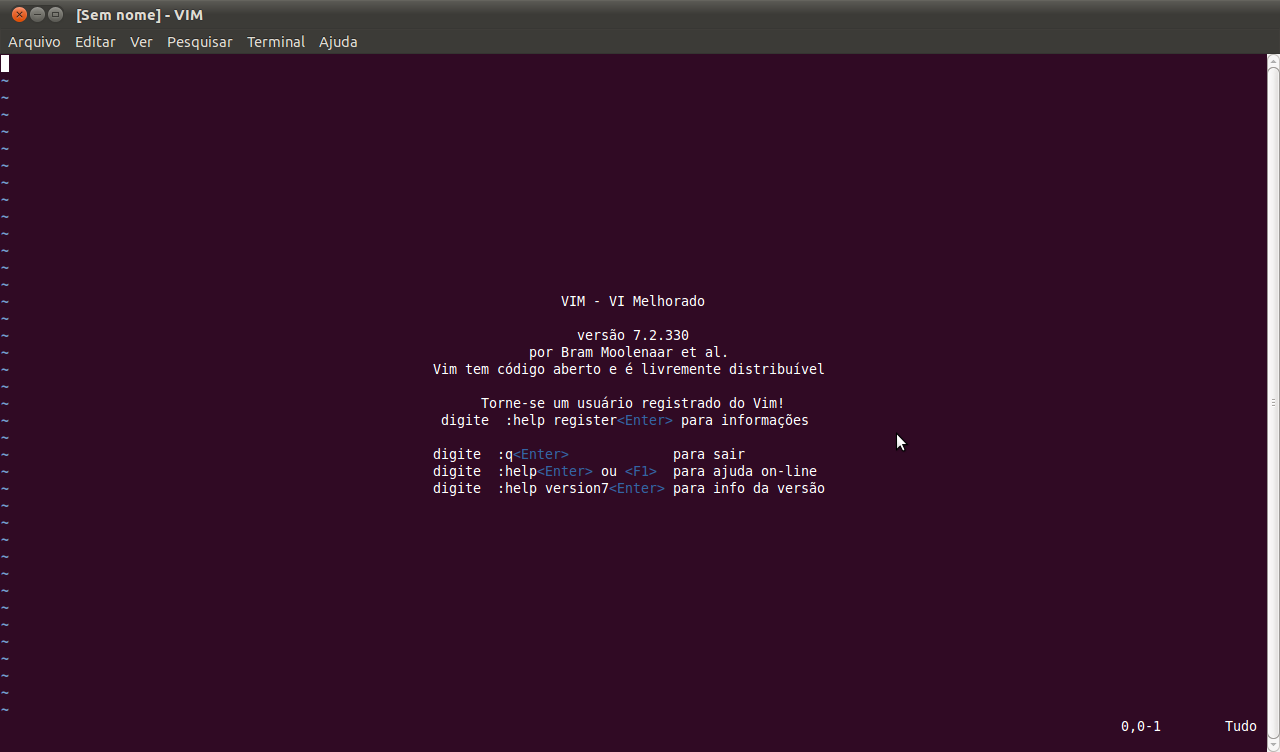
\includegraphics[height=6cm]{figures/vim_screen}
    \caption{Tela inicial do Vim.}
    \label{fig:vim_screen}
\end{figure}

O GVim é uma implemantação do Vim com interface gráfica e na Figura \ref{fig:gvim_screen} encontramos a tela incial do mesmo.
\begin{figure}[h!]
    \centering
    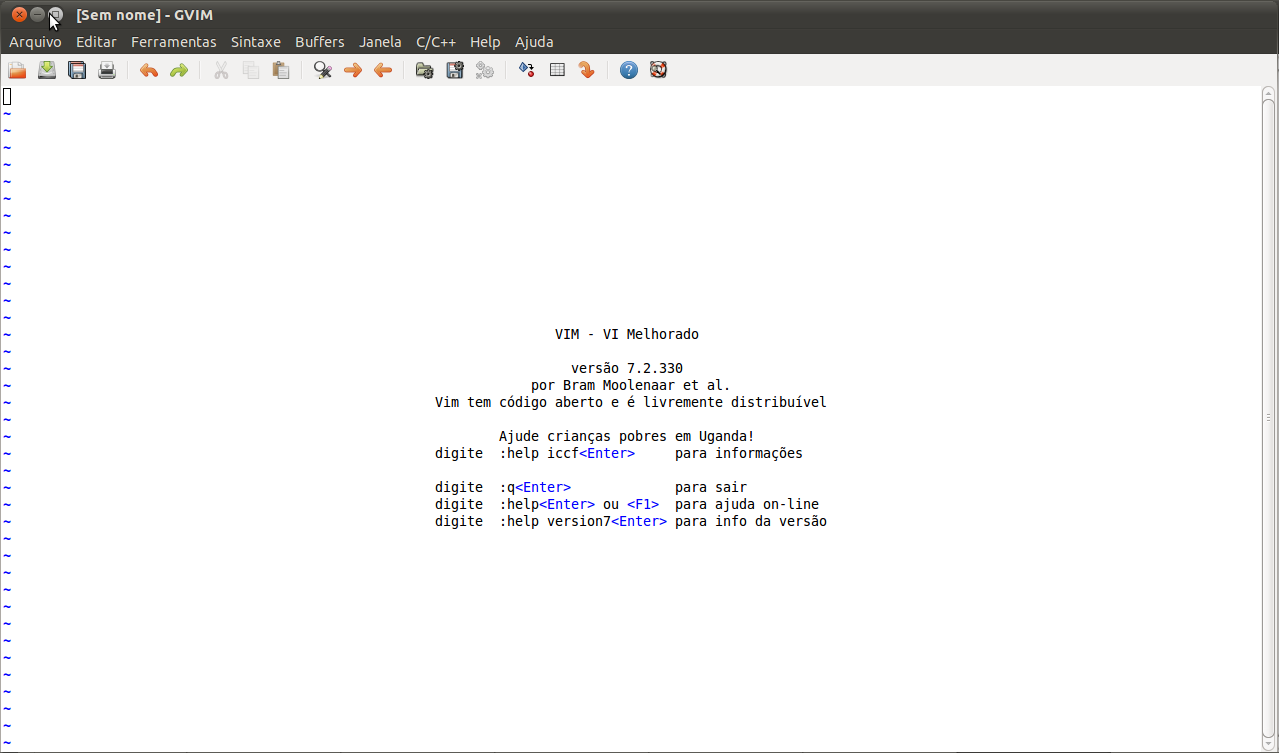
\includegraphics[height=6cm]{figures/gvim_screen}
    \caption{Tela inicial do GVim.}
    \label{fig:gvim_screen}
\end{figure}

\section{Instalação}
\subsection{Windows}

Para a instalação no Windows, versões a partir do XP, pode-se baixar o arquivo disponível em \url{ftp://ftp.vim.org/pub/vim/pc/gvim73_46.exe} e executá-lo.

Destaca-se que uma versão portátil do GVim é encontrada em: \url{http://portablegvim.sourceforge.net/}

\subsection{Linux}

A instalação da distribuição no Ubuntu pode ser feita via terminal com o seguinte comando:
\begin{code}
    sudo apt-get install vim
\end{code}

\section{Iniciando o Vim}

Para iniciar o Vim podemos, a partir da \textit{shell}\footnote{Correspode ao ``prompt de comando'' do usuário}, utiliza-se o comando
\begin{code}
    vim
\end{code}
iniciando o Vim com a tela de boas-vindas ou o comando
\begin{code}
    vim XXX
\end{code}
iniciando o Vim e abrindo o arquivo de texto \lcode{XXX}.

\section{Modos}

No Vim lidamos com dois modos operacionais:
\begin{enumerate}
    \item \textit{Modo de comando};
    \item \textit{Modo de entrada}.
\end{enumerate}

O Vim é iniciado por padrão no \textit{modo de comando} onde cada tecla, ou combinação delas, realizar algum comando. Para alguns comandos precisa-se digitar \lcode{:} , dois pontos, de modo que o cursor muda para o última linha da janela, como apresentado na Figura \ref{fig:vim_colon_screen}. Para que o cursor saia da última linha da janela deve-se precionar a tecla \lcode{Enter}.
\begin{figure}[h!]
    \centering
    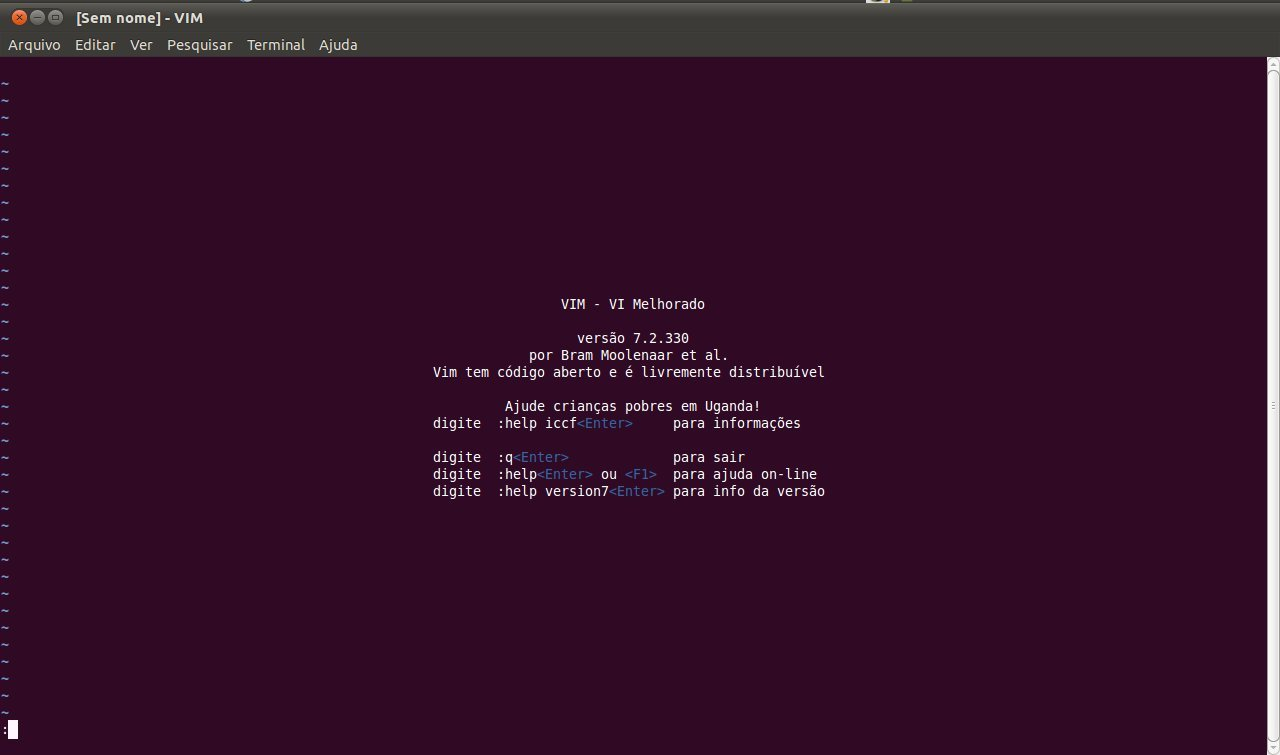
\includegraphics[height=6cm]{figures/vim_colon_screen}
    \caption{Cursor na última linha da janela.}
    \label{fig:vim_colon_screen}
\end{figure}

Já no \textit{modo de entrada}, cada tecla corresponde a uma caractere e é indicado pela presença do texto \lcode{- - INSERÇÃO - -} na última linha da janela, como podemos observar na Figura \ref{fig:vim_insert_screen}.
\begin{figure}[h!]
    \centering
    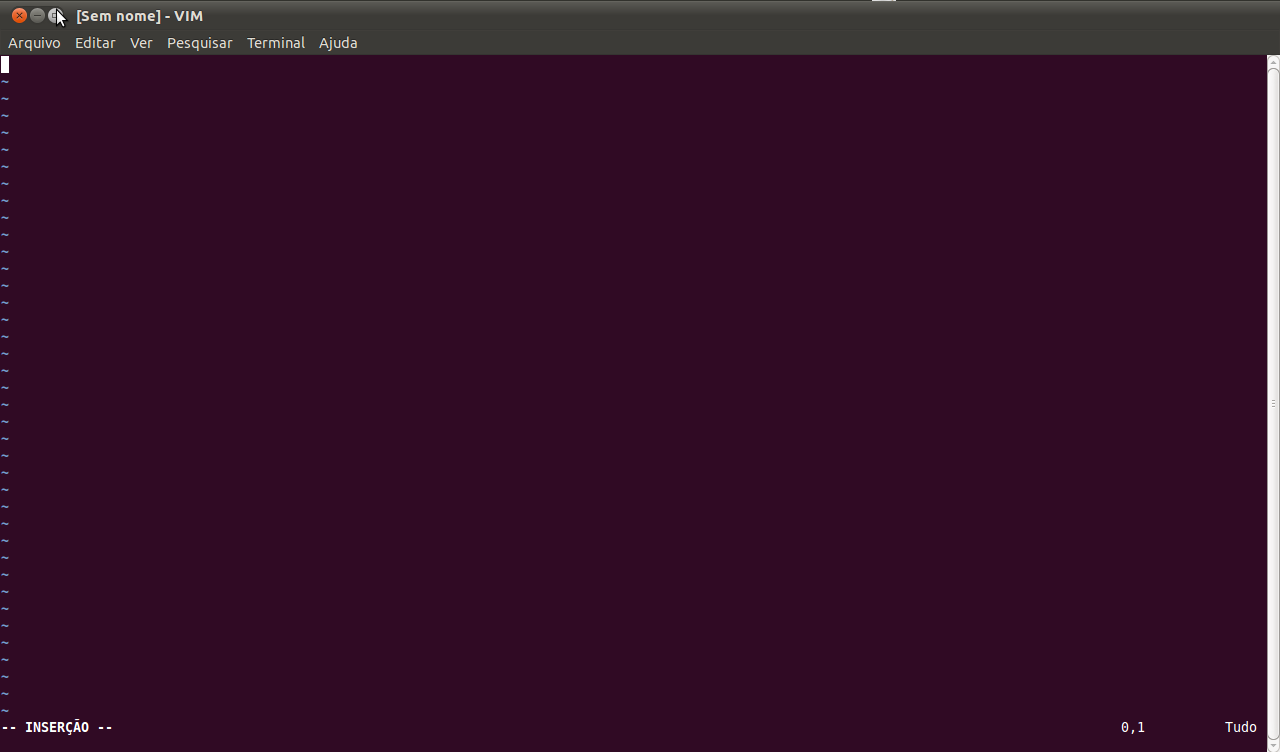
\includegraphics[height=6cm]{figures/vim_insert_screen}
    \caption{Vim no \lcode{modo de entrada}.}
    \label{fig:vim_insert_screen}
\end{figure}
Para mudar do \textit{modo de comando} para o \textit{modo de entrada} deve-se pressionar a tecla \lcode{i} e para retornar a tecla \lcode{Esc}.

Na Figura \ref{fig:vim_modes} observamos como os modos estão relacionados.
\begin{figure}[h!]
    \centering
    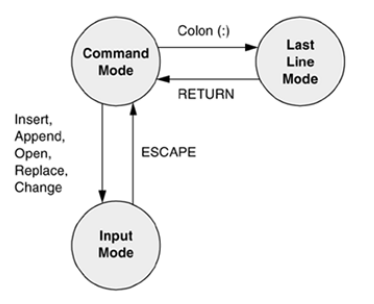
\includegraphics[height=6cm]{figures/vim_modes}
    Fonte: \cite{Sobell:2005:PracticalGuide}
    \caption{Esquema dos modos operacionais do Vim.}
    \label{fig:vim_modes}
\end{figure}

\section{Abrindo um arquivo}
Para abrir um arquivo para edição utiliza-se o comando \lcode{:e} seguido do nome do arquivo a ser editado. Em alguns casos pode ser necessário utilizar o comando \lcode{:e!} ao invés do \lcode{:e} .

\section{Salvando o arquivo}
Para salvar o arquivo atual utiliza-se o comando \lcode{:w}. Em alguns casos pode ser necessário utilizar o comando \lcode{:w!} ao invés do \lcode{:w} .

Caso deseje-se salvar o arquivo atual sem sobrescrever o arquivo existente pode-se utilizar o mesmo comando seguido pelo nome do novo arquivo. 

\section{Fechando o Vim}
Para fechar o Vim deve-se utilizar o comando \lcode{:q} ou \lcode{:q!} para fechar o Vim ignorando as alteração efetuadas no arquivo.

\section{Configuração}

A configuração padrão do Vim, ao ser inicializado, pode ser alterada ao modificar o arquivo \lcode{vimrc}. Nas distribuições Linux deve-se procurar na pasta de usuário pelo arquivo \lcode{.vimrc}, enquanto que no Windows por \lcode{\_vimrc}.

Quando o arquivo \lcode{vimrc} contendo as linhas do código abaixo
\begin{code}
    "Habilita highlight
    syntax on
    "Habilita uso de plugin's dependendo do tipo do arquivo
    filetype plugin on
    "Habilita identacao de acordo com o tipo do arquivo
    filetype indent on
    "Mostra no inicio de cada linha o numero da mesma
    set number
\end{code}
promove o descrito nas linhas iniciadas com aspas\footnote{Nos arquivos utilizados pelo Vim, linhas iniciadas por aspas são comentários e por isso ignoradas pelo Vim.}.

Para outras configurações sugere-se olhar os seguintes endereços:
\begin{itemize}
    \item \url{http://aurelio.net/doc/dotfiles/vimrc.txt}
    \item \url{http://aurelio.net/vim/vimrc-voyeg3r.txt}
    \item \url{http://aurelio.net/vim/vimrc-ivan.txt}
\end{itemize}

\section{Ajuda}

A ajuda no Vim pode ser obtida pelo comando \lcode{:help} .
